\documentclass{standalone}
\usepackage{pgfplots}
\pgfplotsset{compat=newest}
\begin{document}
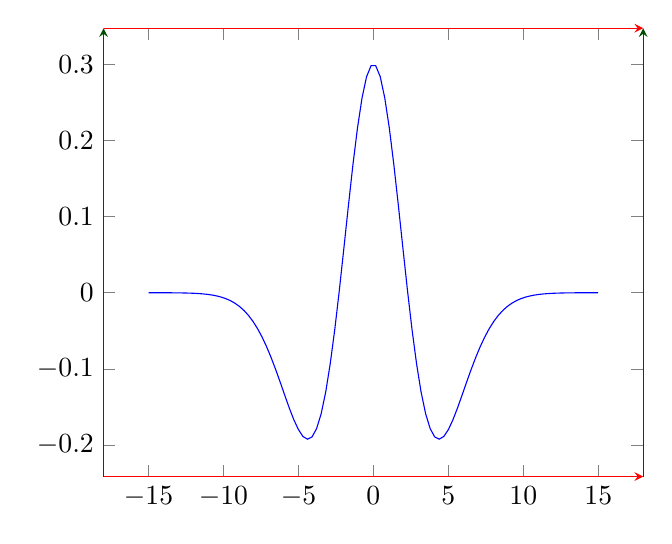
\begin{tikzpicture}
\begin{axis}[
	separate axis lines,
	every outer x axis line/.append style=
		{-stealth,red},
	every outer y axis line/.append style=
		{-stealth,green!30!black},
]
\addplot[blue,
		samples=100,
		domain=-15:15] 
	{1.3*exp(0-x^2/10) - exp(0-x^2/20)};
  % Unfortunately, there is a bug in PGF 2.00
  % something like exp(-10^2)
  % must be written as exp(0-10^2) :-(
\end{axis}
\end{tikzpicture}
\end{document}
